% Gerado por scripts/generate_posthoc_fragment.py; não editar à mão.
\label{sec:calibracao}

The MLE was fitted on the 1,063 windows of 1,000 events
in the \texttt{calibration\_train} block (15 to 22 January 2024), the only
block authorized for calibration. The median $\beta$ was 2.71 (interquartile
range 2.21--3.14), above the upper limit of 2.0 used in training, and
$\alpha_{\mathrm{cross}}$ was below $10^{-3}$ in 89.4\% of the windows.
Only 15.4\% of the windows have $\beta$ inside the
prior, 0.4\% have the self-excited fraction
inside $[0.2,\,0.8]$, and 0.0\% satisfy all the ranges at once.
Because an estimator trained with quadratic loss approximates the posterior
mean under the training prior, the current networks cannot produce estimates
in this region; the empirical evaluation requires recalibrating the prior or
training on MLE labels from real windows.

\begin{figure}[htbp]
\centering
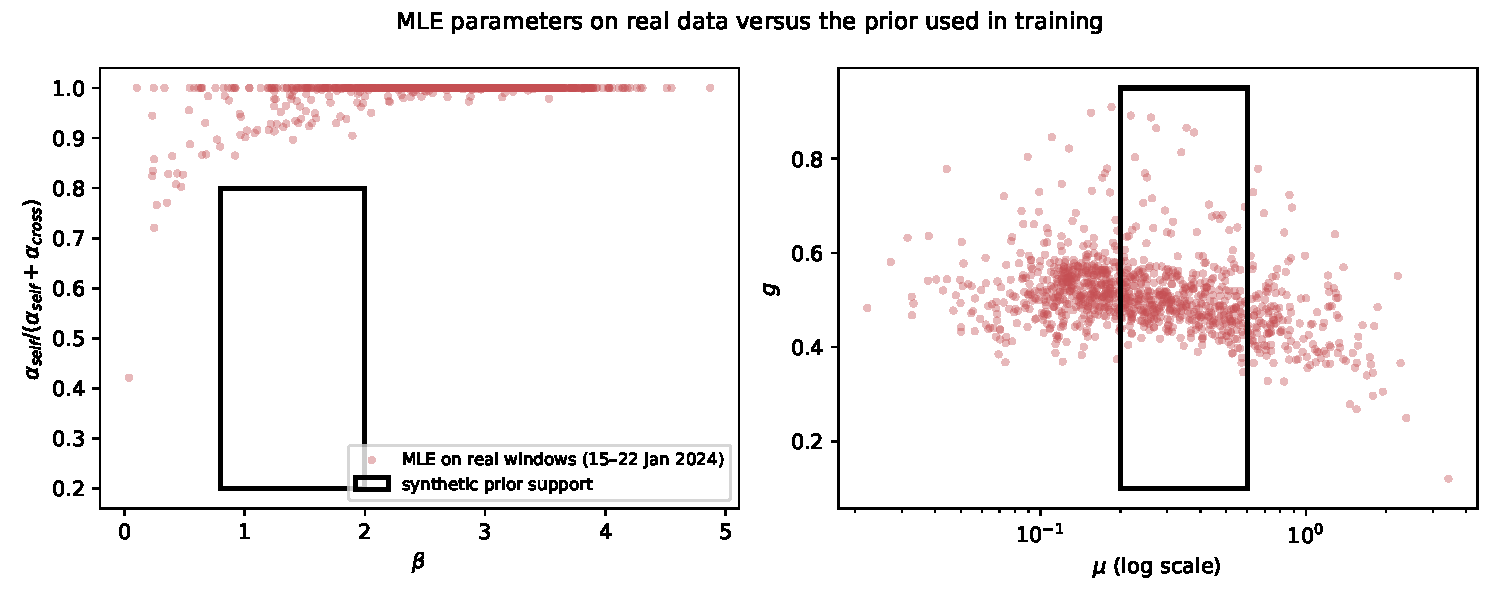
\includegraphics[width=0.95\linewidth]{../build/figures/posthoc_calibracao_vs_prior_en.pdf}
\caption{MLE estimates on the real calibration windows (points) and support
of the prior used to generate the training data (rectangles).}
\label{fig:calibracao-prior}
\end{figure}
